\section{Encoding Ordered Attributes} 
\label{sec:ordering}
Until now, we have assumed every attribute set is an unordered collection: the network does not prefer any attribute over another, and does not check the attributes in any deliberate order. However, this is not true for many applications of interest, including our example of service chaining. Operators expect middleboxes to be visited in a specific order to ensure correctness or performance guarantees. In this section, we cover how our encoding scheme can be adapted to support ordered attribute \textit{sequences}.


\subsection{Total Orderings}
\begin{figure}
    \begin{tabular}{| l | l | l |}
    \hline
    Attribute & Unordered Match & Ordered Match\\ \hline
    A & $1011**$ & $1011**$ \\ \hline
    B & $101*1*$ & $10101*$ \\ \hline
    C & $101**1$ & $101001$ \\
    \hline
    \end{tabular}
    \caption{This table shows how the wildcard strings differ for ordered versus unordered attributes, using the example superset $(A,B,C)$ with identifier $101$. In the unordered case, the string matches if the target attribute bit is 1, and does not depend upon the bits of other attributes. In the ordered case, the string only matches if the target attribute bit is 1 and all bits for attributes preceding the target attribute are 0. This ensures only matching on the attribute earliest in the ordering succeeds.} 
    \label{tab:ordering}
\end{figure}


It is possible to maintain the ordering upon the attributes encoded by the tags. Figure \ref{tab:ordering} shows how the wildcard strings can be modified to impose an ordering upon the elements. If the ordering dictates that $X$ must appear before $Y$, then any wildcard string for decoding $X$ must check that the $X$ bit is 1 and the $Y$ bit is 0. This causes the wildcard string to only successfully match if no other attributes that come before $X$ appear in the set. In other words, testing for $X$ only returns true if tests for all attributes before $X$ returns false. 

However, this only works if all attribute sequences are drawn from a \textit{total ordering}. That is, if attribute $X$ appears before $Y$ in any sequence, then $X$ must appear before $Y$ in all sequences. If we have the two sequences $(X, Y)$ and $(Y, X)$, this approach immediately breaks.

\subsubsection{Partial Ordering}
Not all is lost if the attributes are not totally ordered. If attribute $X$ appears before $Y$ in some sequences, but $Y$ appears before $X$ in others, then $X$ and $Y$ are an \textit{incomparable} pair. If there are only a few incomparable pairs, then the universe is \textit{partially ordered}. It is still possible to encode such a list of sequences using our scheme, but at the cost of increased tag width.

Consider the case of an incomparable pair $(X,Y)$. We can 'split' $X$ into two different attributes, $X_1$ and $X_2$. For every sequence where $X$ appears before $Y$, we replace $X$ with $X_1$. If $X$ appears after $Y$, we replace $X$ with $X_2$. The result is a new universe of attributes which has the total ordering $(X_1, Y, X_2)$. 

This fix comes at a cost, however. The number of attributes we must encode increases for every incomparable pair that must be resolved. Additionally, it is unclear how to resolve all conflicts using a minimal number of splits. In fact, if we generalize the problem slightly to allow attributes to appear more than once per sequence, the problem becomes the Shortest Common Supersequence problem. This problem is well known to be NP-Hard, even for the simple case of only two attributes! As a result, we cannot hope to optimally minimize the number of attribute splits needed to resolve all incomparabilities, but we can attempt to heuristically minimize them.

\subsection{Partial to Total Ordering}
In this section, we present a heuristic algorithm for resolving incomparabilities.
 Figure \ref{fig:ordering} shows our heuristic for choosing a set of attributes to split which attempts to minimize the number of splits. For a concrete example, we are given four input sequences we wish to encode, shown in \ref{fig:ordering}(a). We assume that these sequences \textit{almost} follow an underlying ordering, but that there are a few incomparable sets of elements. In this example, $B$ is incomparable with $C$ because $B$ appears both before and after $C$. 

To systematically identify these incomparable elements, we construct the sequence graph, shown in \ref{fig:ordering}(b). In the sequence graph, element $u$'s node has an edge to element $v$'s node if $u$ appears before $v$ in any sequence. We then run an algorithm for finding Strongly Connected Components (SCCs) on this graph. A strongly connected component is a set of nodes such that for every pair of nodes $u$ and $v$ in the set, $u$ has a path to $v$ and vice versa. In this context, every SCC corresponds to a set of incomparable elements. Figure \ref{fig:conflict_res} shows the process for determining which elements to split to create a new, totally ordered universe. Figure \ref{fig:ordering}(d) and (e) shows the result of using this new ordering to modify each sequence. 


\begin{figure}[t!] 
\begin{minipage}{1\linewidth}
\begin{subfigure}[c]{0.96\linewidth}
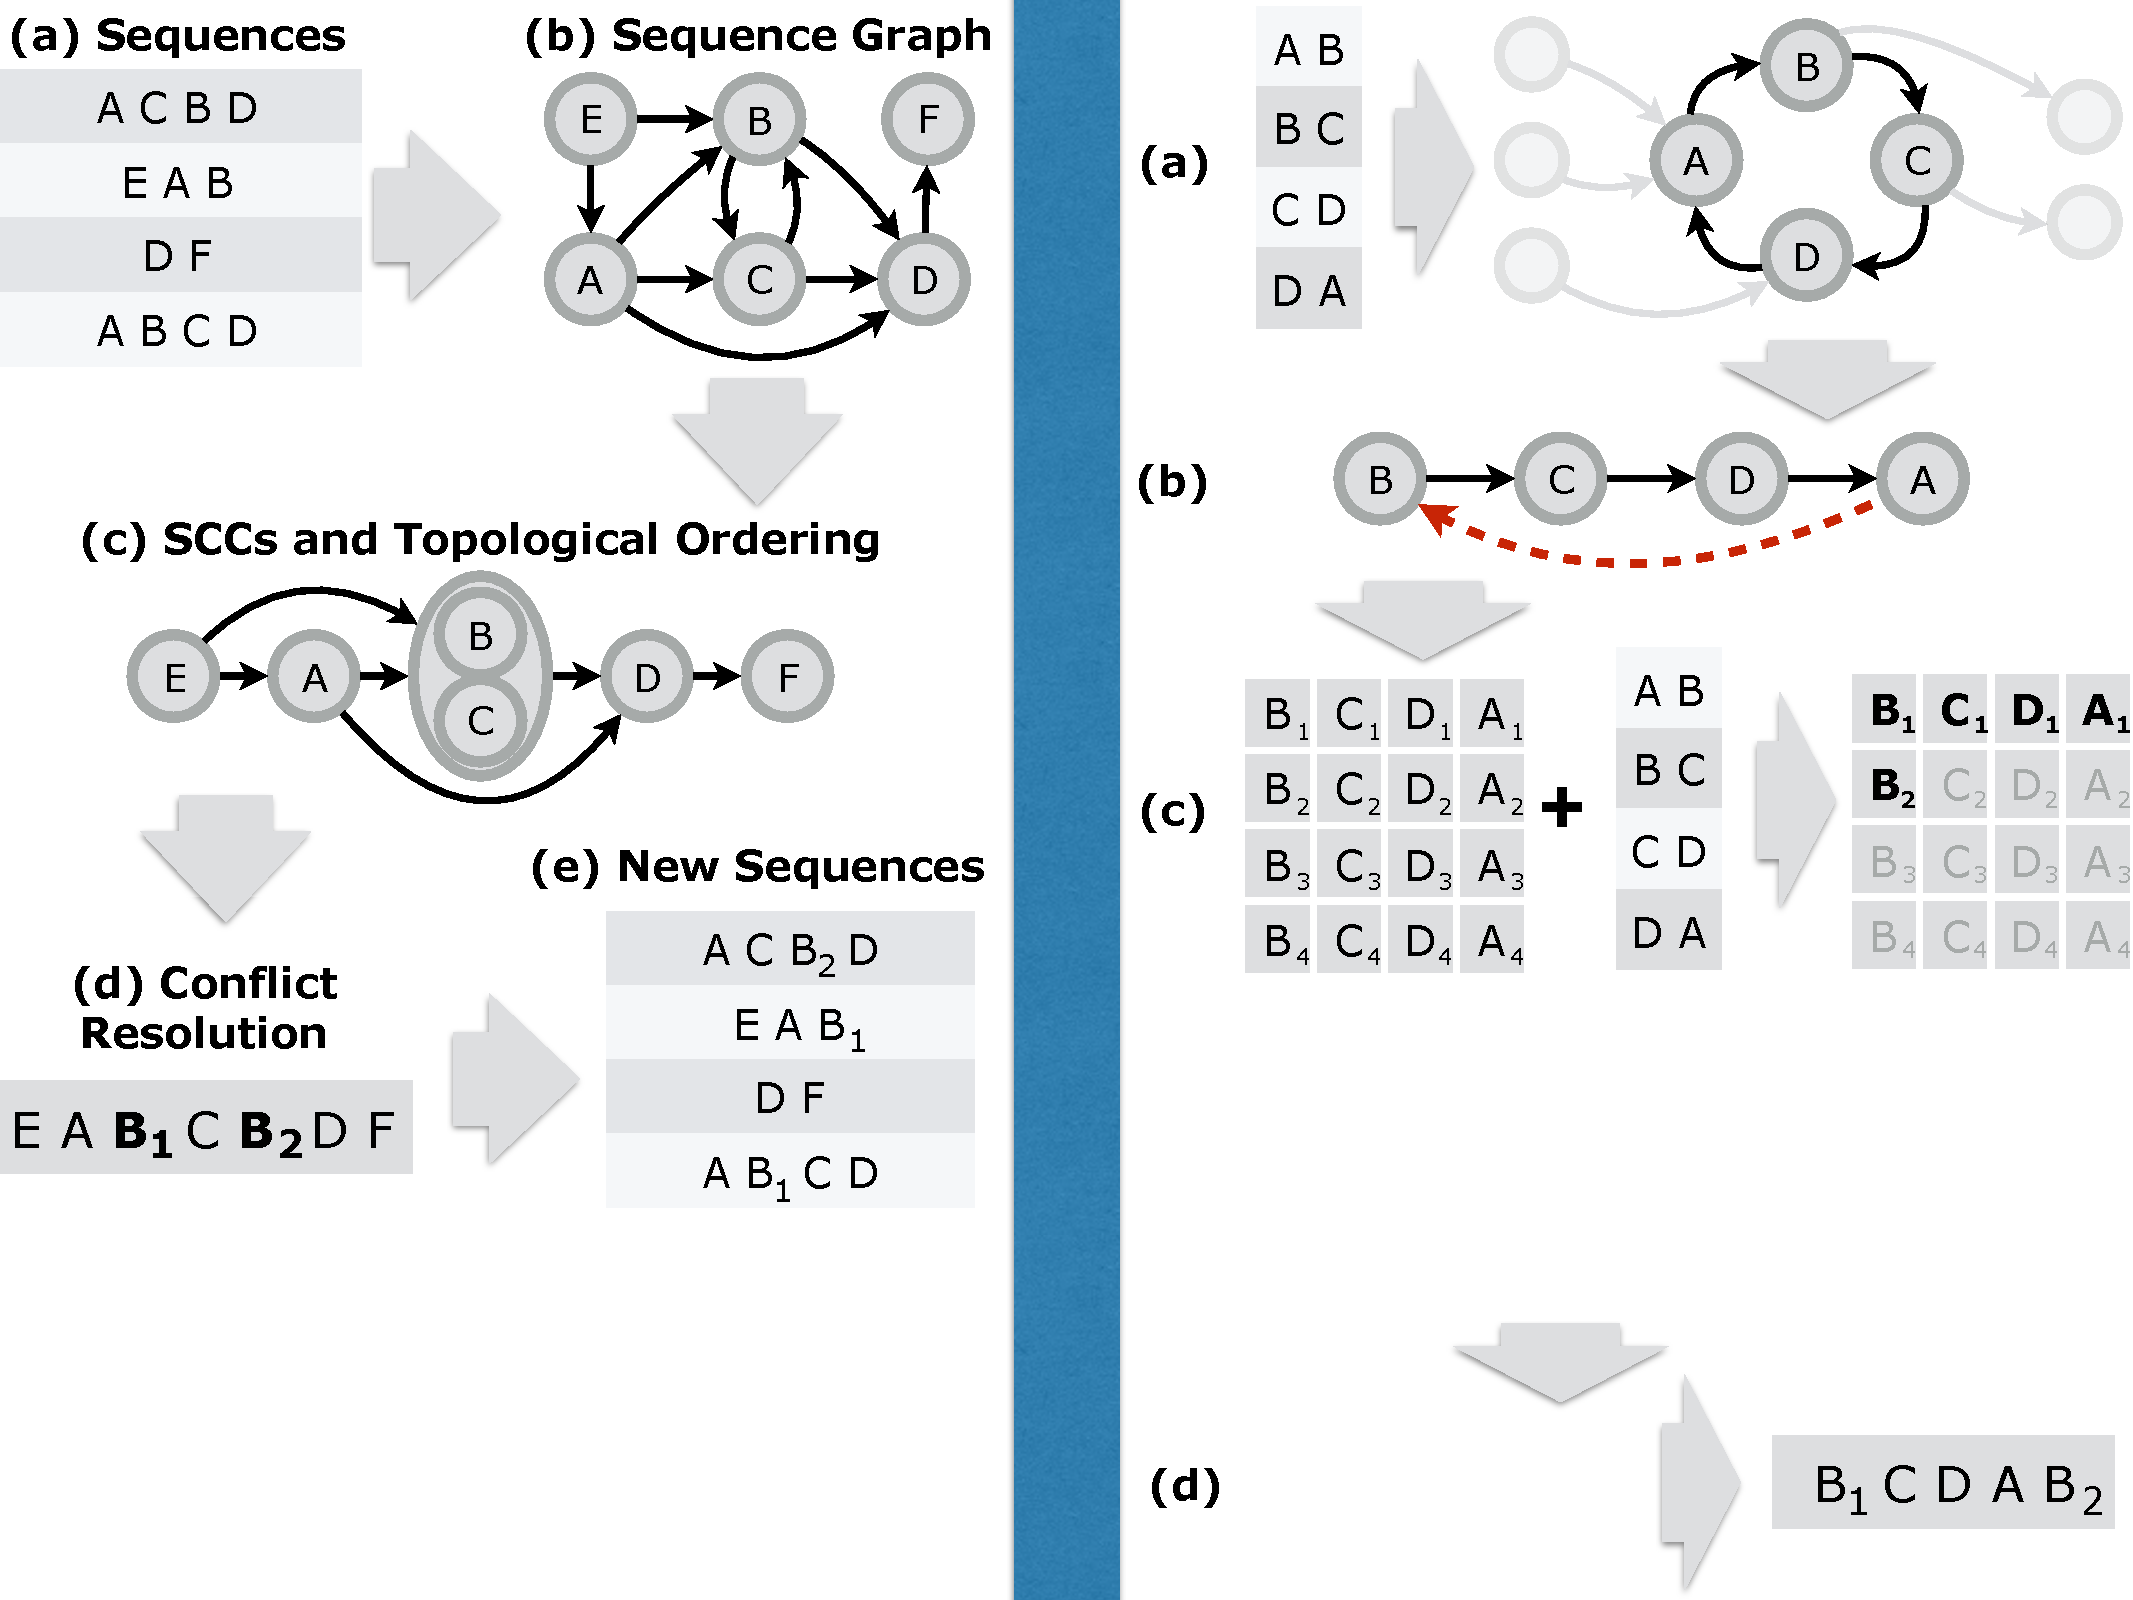
\includegraphics[trim={0 6cm 19.2cm 0}, clip, width=\linewidth]{figures/partial_ordering}
\end{subfigure} 
\end{minipage} 
\caption{This figure shows, at a high level, the process for converting a partial ordering to a total ordering by identifying incomparable elements and creating duplicates to resolve the incomparabilities. (a) shows the four input ordered sequences. In (b), we create a graph of the elements, where there is an edge from $u$ to $v$ if $u$ appears before $v$ in some sequence. (b) shows how the graph can be broken up into an ordered Directed Acyclic Graph (DAG) of Strongly Connected Components (SCC), where each SCC corresponds to a set of incomparable elements. (d) shows the result of splitting elements to resolve incomparability, which is covered in more depth in figure \ref{fig:conflict_res}. In (e), the original sequences are modified with the splits such that each sequence adheres to a total ordering.}
\label{fig:ordering}
\end{figure}



\begin{figure}[t!] 
\begin{minipage}{1\linewidth}
\begin{subfigure}[c]{0.96\linewidth}
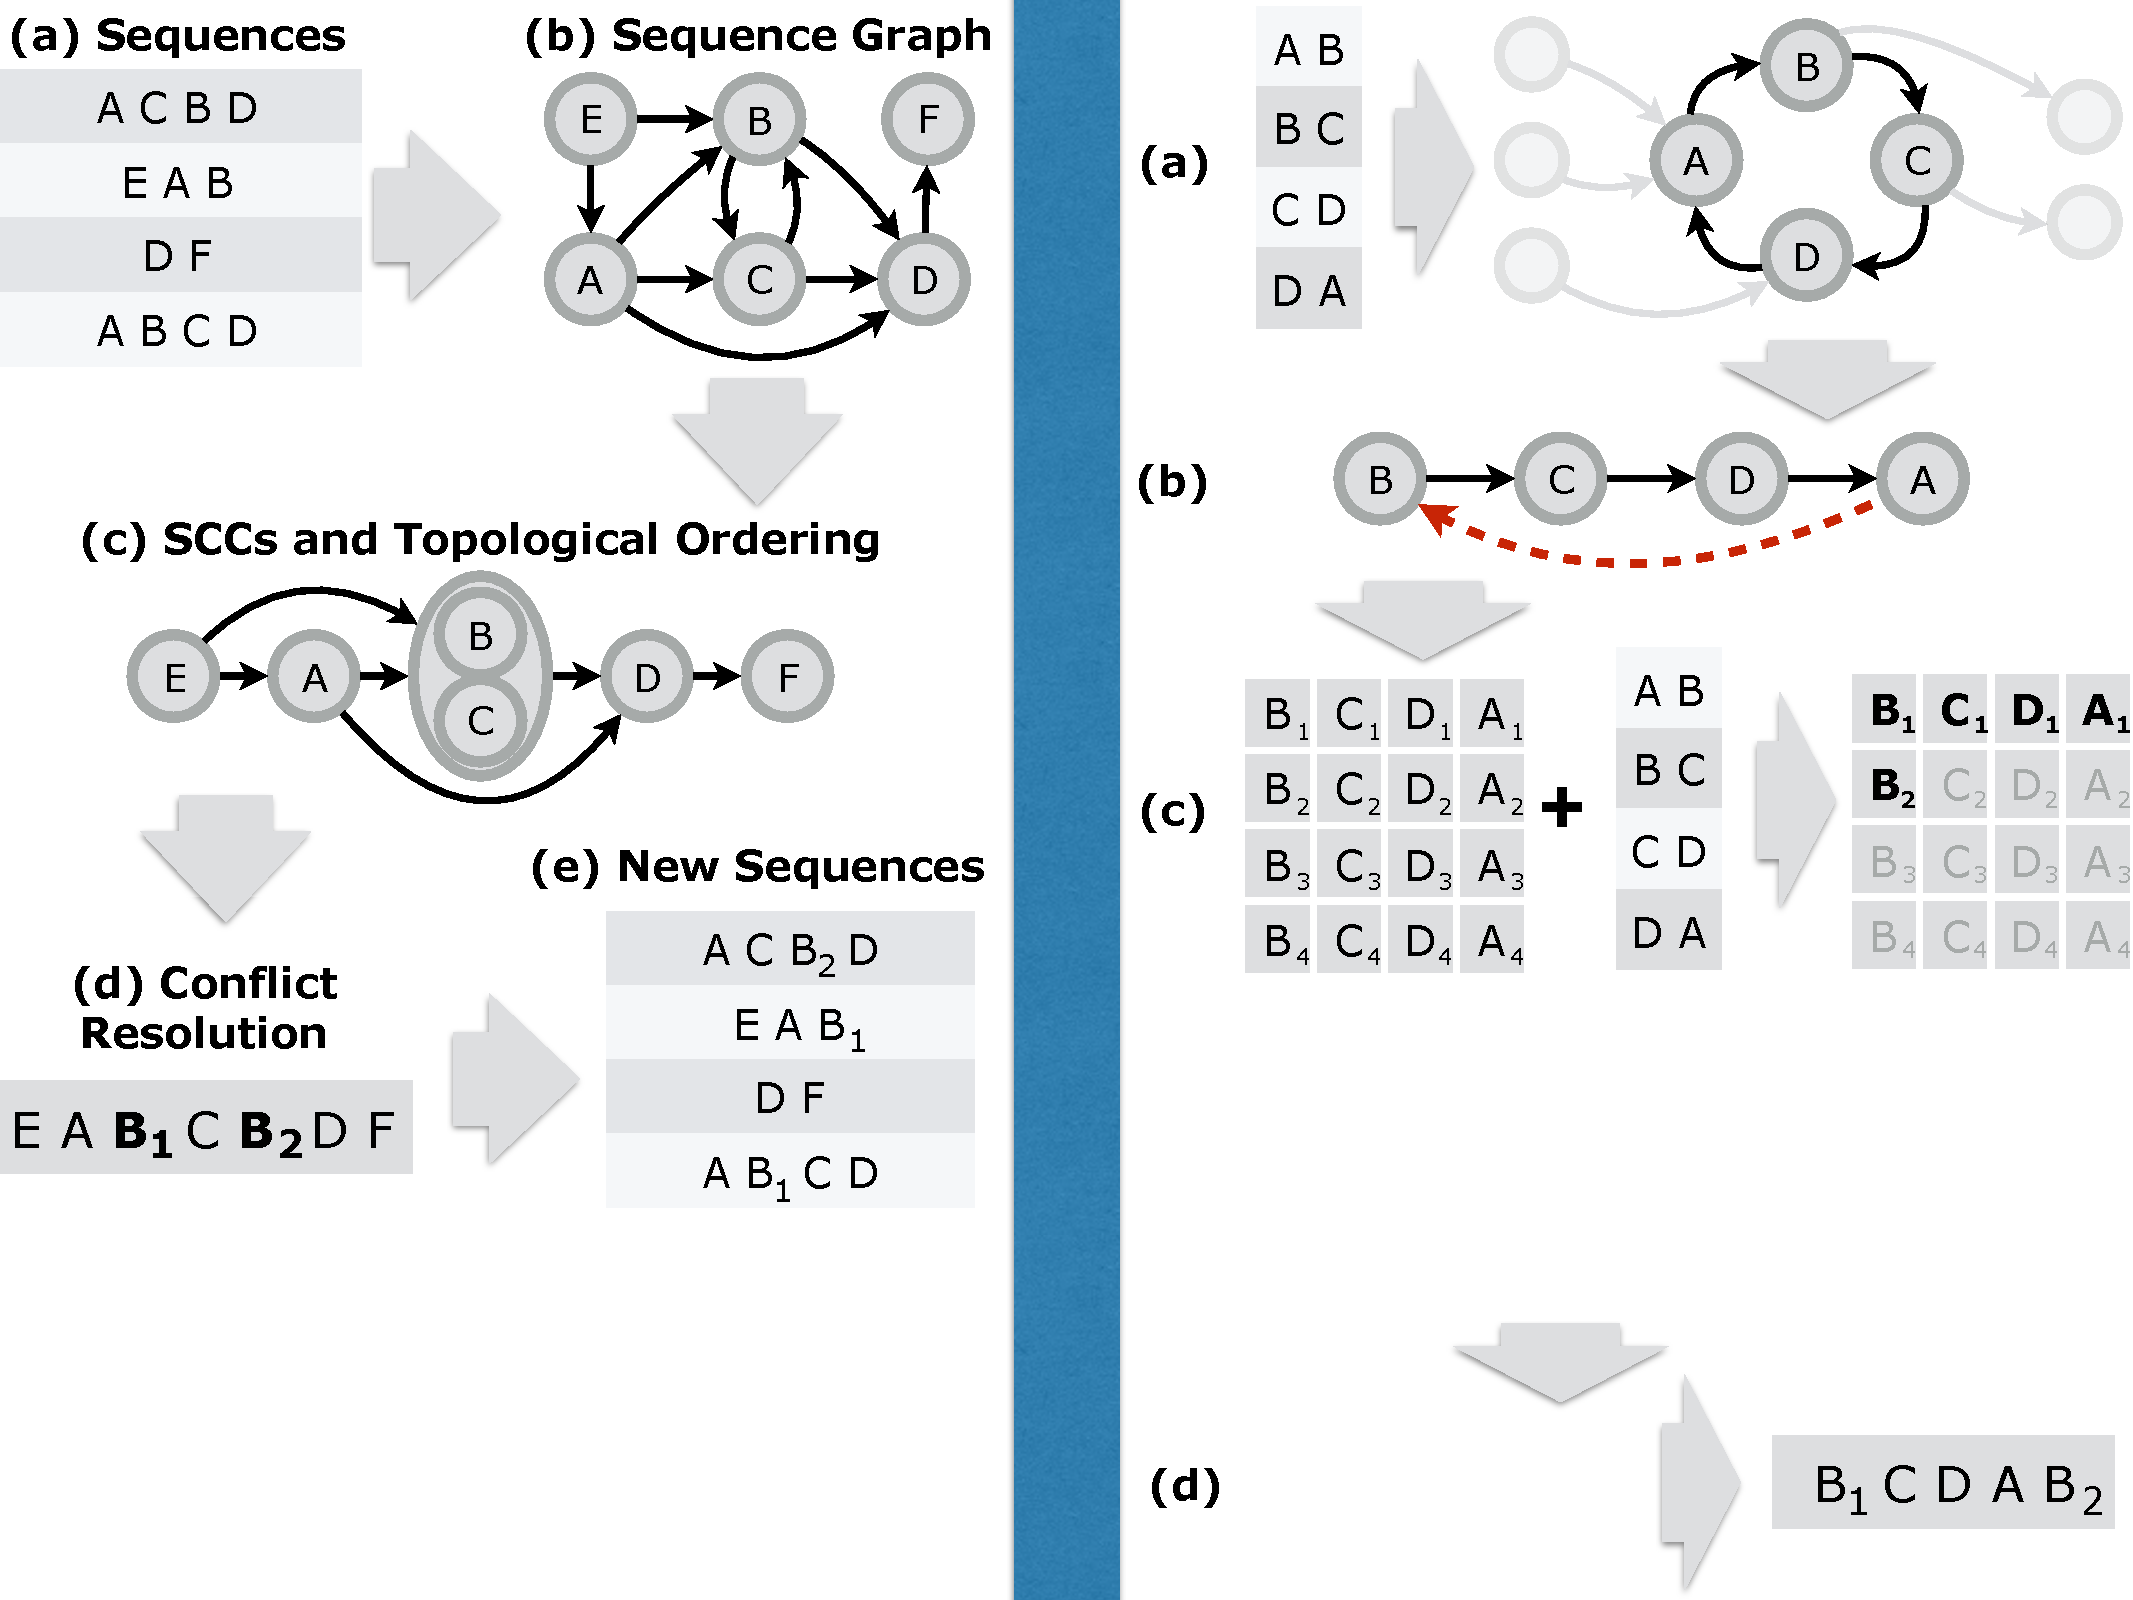
\includegraphics[trim={19.2cm 10cm 0 0}, clip, width=\linewidth]{figures/partial_ordering}
\end{subfigure} 
\end{minipage} 
\caption{This details the Conflict Resolution step of the algorithm. (a) shows a SCC corresponding to four incomparable elements. (b) shows an 'almost' ordering of the SCC nodes, which minimizes the number of backward edges. (c) shows how the almost ordering is used to construct a worst-case quadratically-sized universe, which is then traversed by every sequence to determine which splits are necessary. }
\label{fig:conflict_res}
\end{figure}

